\documentclass[12pt]{article}
\usepackage[czech]{babel}
\usepackage[utf8]{inputenc}
\usepackage[plainpages=false,pdfpagelabels,unicode]{hyperref}
\usepackage[pdftex]{graphicx}
\usepackage[margin=2cm, includefoot]{geometry}

\begin{document}

\title{Praktikum z fyziky plazmatu \\
Studium kladného sloupce doutnavého výboje pomocí elektrostatických sond}
\author{Pavel Ondračka}
\maketitle

\section{Úvod}
Sondou všeobecně rozumíme vodič malých rozměrů vnořený do plazmy za účelem získání nějaké fyzikální veličiny. Nejčastěji se používají vodiče tvaru destičky, válce a koule. Dále rozlišujeme sondy jednoduché a dvojné. V tomto praktiku byly použity jednoduchá rovinná a dvojná válcová sonda.

\subsection{Jednoduchá rovinná sonda}
Z naměřené voltampérové charakteristiky stanovíme elektronový proud $I_\mathrm{e}$ odečtením iontového proudu. Ten určíme v oblasti čistě iontového proudu (pro nízké napětí) nafitováním přímky.

 Sestrojíme závislost $\mathrm{ln}\,I_\mathrm{e} = -\frac{e}{k T_\mathrm{e}}U + C$. Potenciál plazmatu $U_\mathrm{p}$ určíme ze zlomu této závislosti jako průsečík asymptot k lineárním částem charakteristiky. Směrnice asymptoty $a$ pod potenciálem plazmatu určuje elektronovou teplotu $T_\mathrm{e}$
\begin{equation}
T_\mathrm{e} = \frac{e}{k} \frac{1}{a} \mathrm{.}
\end{equation}

Koncentrace elektronů určíme z elektronového proudu sondou $I_\mathrm{e}$ v případě $U_\mathrm{p}$ = $U_\mathrm{s}$, pak platí
\begin{equation}
n_\mathrm{e} = \frac{I_\mathrm{e}}{S e} \sqrt{\frac{2 \pi m}{k T_\mathrm{e}}} \mathrm{,}
\end{equation}
kde $S$ je plocha sondy. Schéma zapojení pro měření jednoduché sondové VA charakteristiky je na~obrázku \ref{schemajednoducha}. 

\begin{figure}[htbp]
\begin{center}
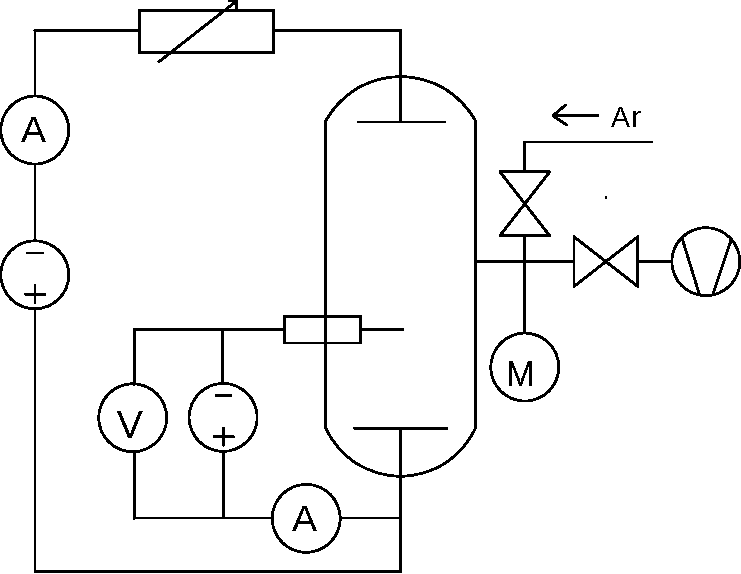
\includegraphics[width=10cm]{schemajednoducha.pdf}
\caption{Schéma zapojení aparatury pro jednoduchou sondu}
\label{schemajednoducha}
\end{center}
\end{figure}

\subsection{Dvojná válcová sonda}
Dvojnou symetrickou sondou rozumíme dvě stejné sondy, umístěné v ekvipotenciální ploše v~plaz\-ma\-tu. Žádná z těchto sond není spojena s elektrodou, ustavují se tedy bez vnějšího zdroje na plovoucím potenciálu $U_\mathrm{fl}$. Studium plazmatu pomocí dvojné sondy provádíme tak, že měříme cirkulační proud $I_\mathrm{d}$ okruhem sond po přivedení napětí $U_\mathrm{d}$ mezi sondy. Pro elektronovou teplotu platí
\begin{equation}
T_\mathrm{e} = 11600 (G - G^2) R_0 \sum{I_\mathrm{p}} \mathrm{,}
\end{equation} 
kde $R_0 = \frac{\mathrm{d}U_\mathrm{d}}{\mathrm{d}I_\mathrm{d}}|_{U_\mathrm{d}=0}$, $\sum{I_\mathrm{p}} = I_\mathrm{p1} + I_\mathrm{p2}$ v bodě $\alpha$, $G = \frac{I_\mathrm{e2}}{\sum{I_\mathrm{p}}}|_{U_\mathrm{d}=0}$. Veličiny $I_\mathrm{p1}$, $I_\mathrm{p2}$, $I_\mathrm{e2}$, $\mathrm{d}U_\mathrm{d}$ a $\mathrm{d}I_\mathrm{d}$ jsou vyznačeny na obrázku \ref{sonda2graf}. Zapojení aparatury pro měření dvojnou sondou je na obrázku \ref{schemadvojita}.

\begin{figure}[htbp]
\begin{center}
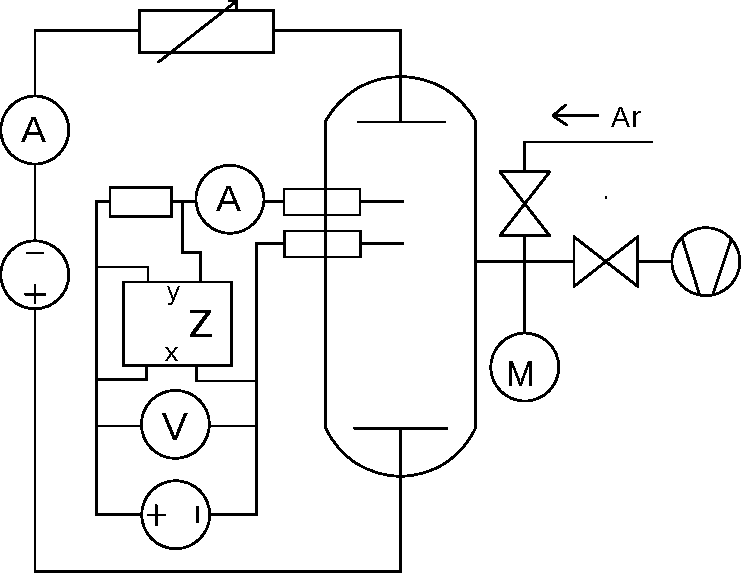
\includegraphics[width=10cm]{schemadvojita.pdf}
\caption{Schéma zapojení aparatury pro dvojnou sondu, Z -- zapisovač}
\label{schemadvojita}
\end{center}
\end{figure}

\begin{figure}[htbp]
\begin{center}
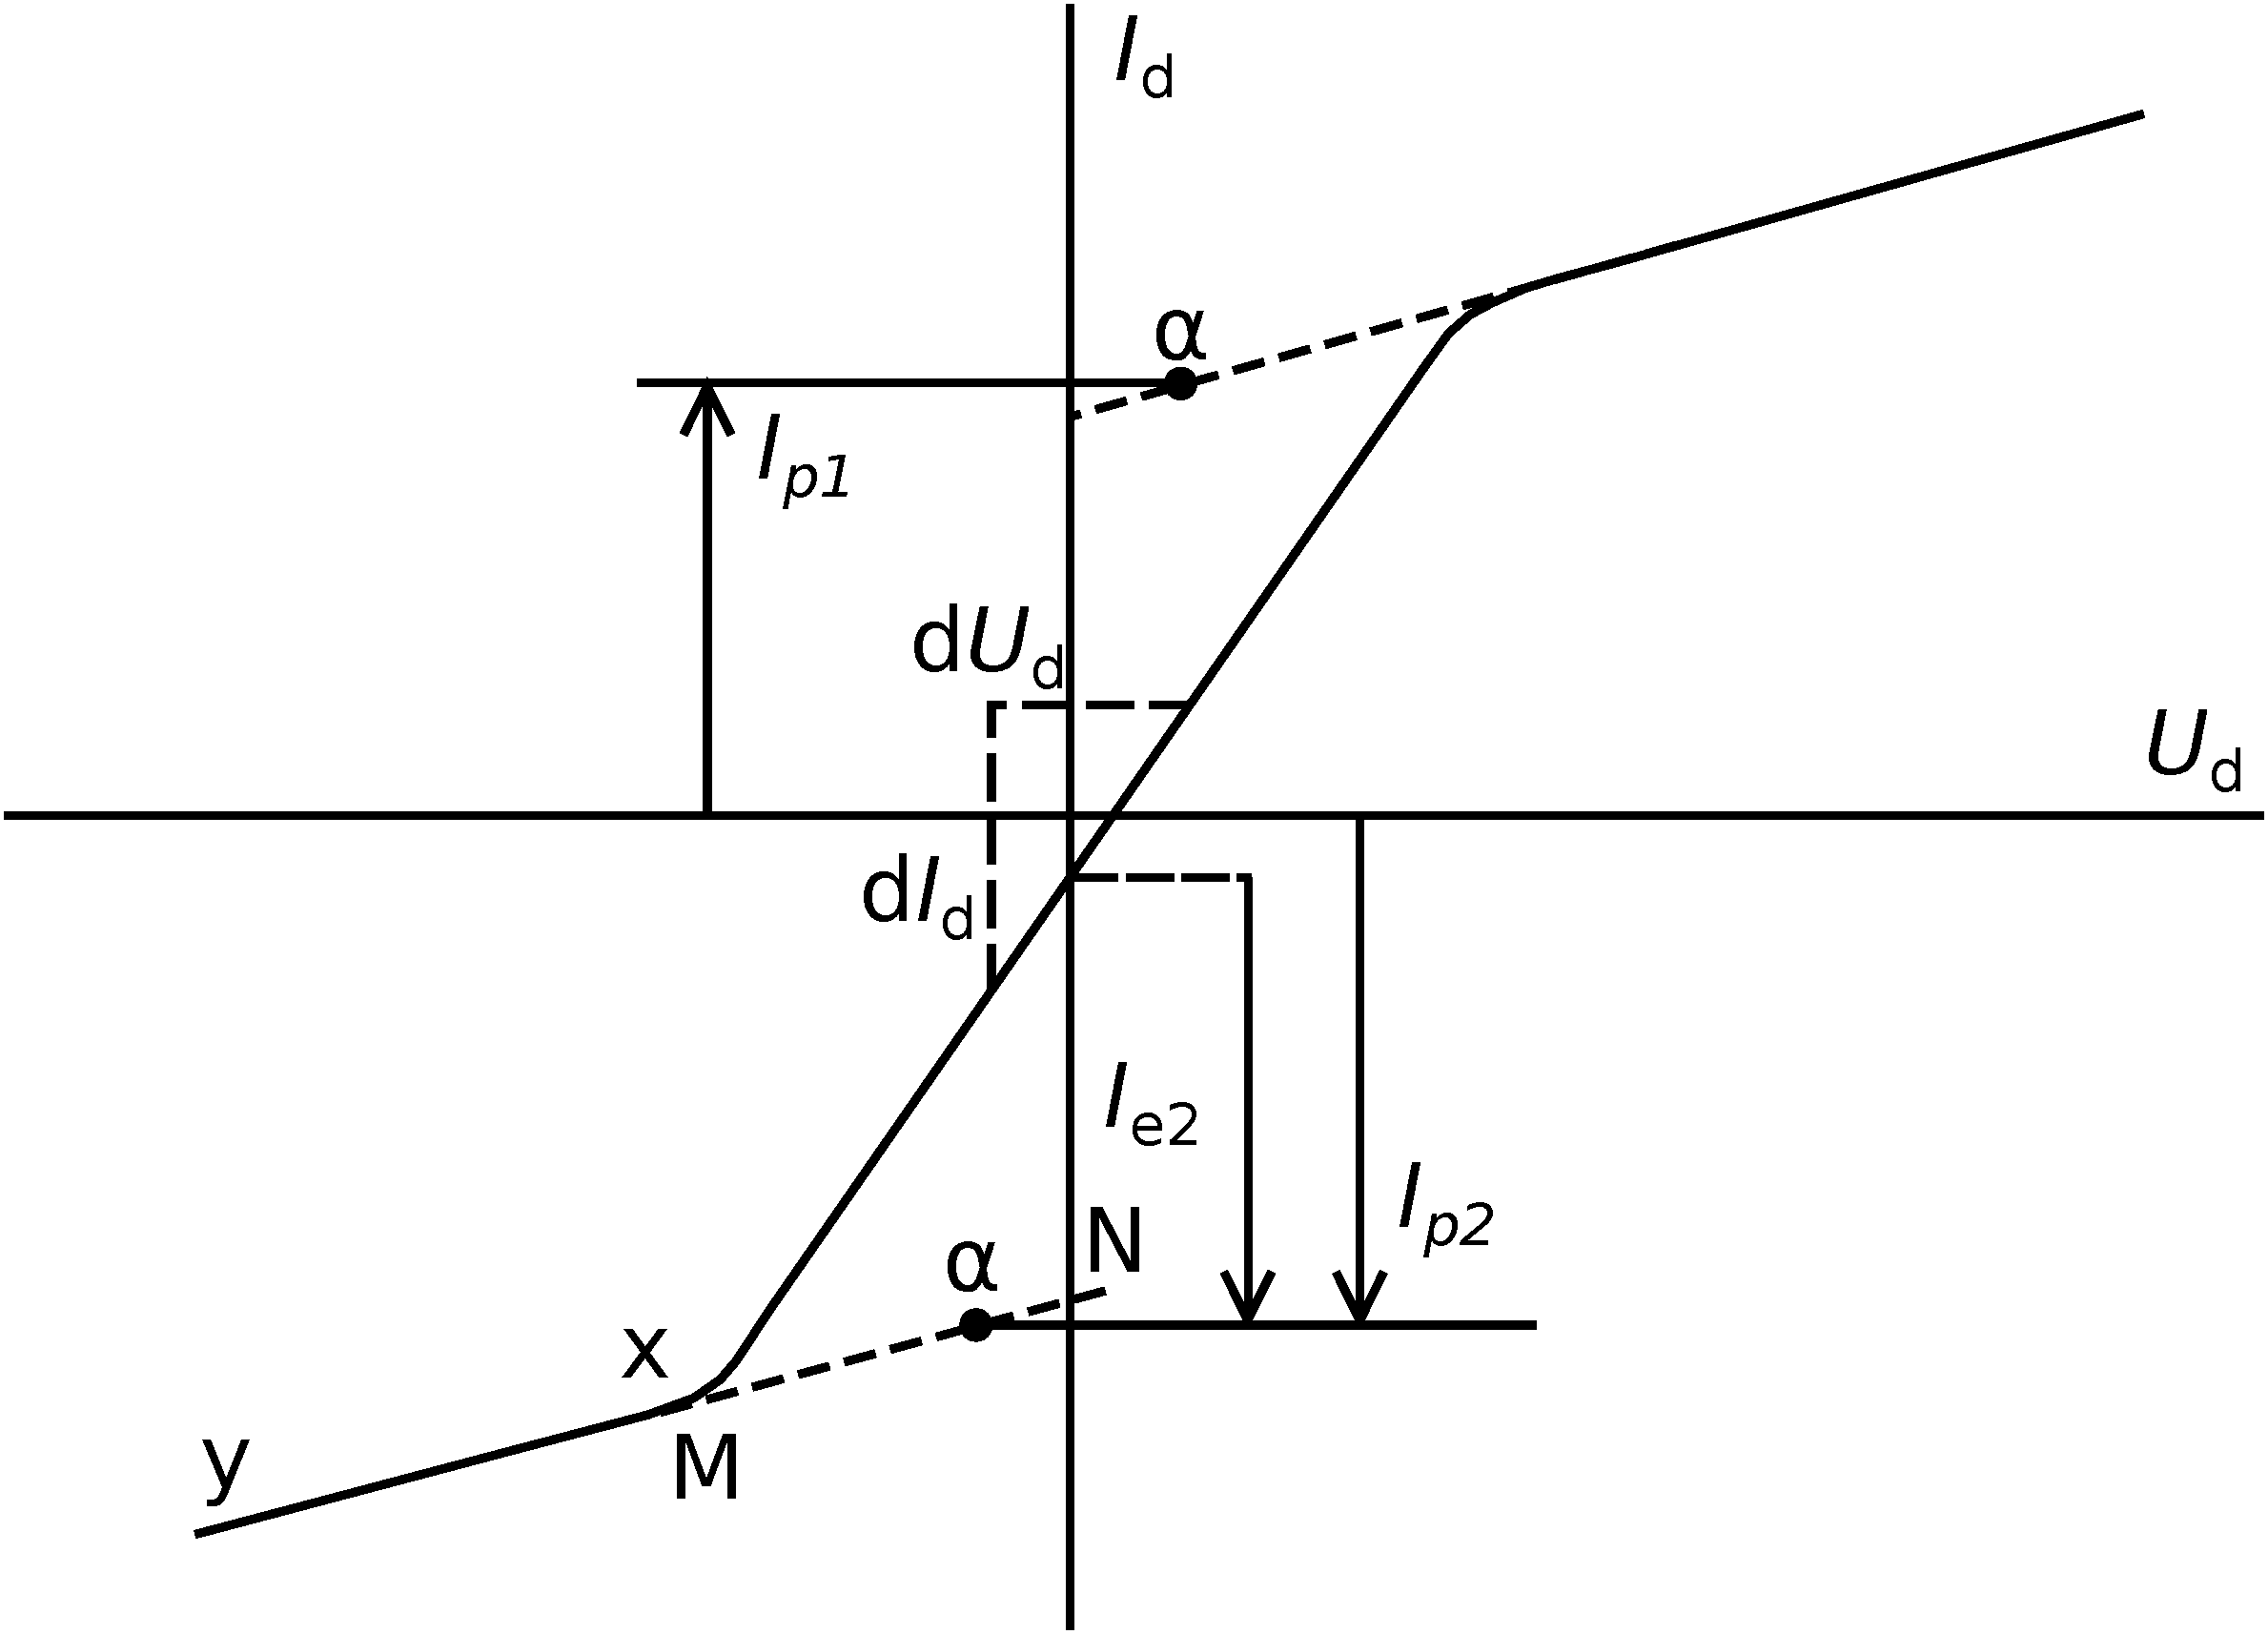
\includegraphics[width=12cm]{sonda2graf.pdf}
\caption{Stanovení $I_\mathrm{p1}$, $I_\mathrm{p2}$, $I_\mathrm{e2}$, $\mathrm{d}U_\mathrm{d}$ a $\mathrm{d}I_\mathrm{d}$ z naměřené VA charakteristiky}
\label{sonda2graf}
\end{center}
\end{figure}

\section{Měření}
\subsection{Jednoduchá rovinná sonda}
VA charakteristika sondy byla měřena pro dva výbojové proudy: 45\,mA a 31\,mA. Naměřené proudy sondou s nafitovanými iontovými proudy a elektronovými proudy jsou na obrázcích \ref{iv45} a \ref{iv31}. Zlogaritmované elektronové proudy s vyznačeným potenciálem plazmatu a asymptotami jsou na obrázcích \ref{ln45} a \ref{ln31}. Použitá rovinná sonda má tvar kruhu s průměrem $d=2\pm1\,\mathrm{mm}$ a plochou $S=3,14\pm3,14\,\mathrm{mm^2}$. Průměr sondy byl určen odhadem, chybu jsem odhadl na 50\,\%. 
Během určování potenciálu plazmatu se vyskytlo několik problémů. Jednak se ukázalo, že potenciál plazmatu je pod plovoucím potenciálem, což neodpovídá teorii, navíc bylo poměrně obtížné určit přesnou polohu potenciálu plazmatu protože logaritmus elektronového proudu pod zlomem závislosti není moc lineární, tj. velmi záleží na výběru oblasti pro fitování asymptoty. Chybu plovoucího potenciálu jsem proto odhadl na $\pm0,5\,\mathrm{V}$, chyba elektronového proudu $I_\mathrm{e}$ v bodě $U_\mathrm{p}$ = $U_\mathrm{s}$ byla pak určena jako polovina změny elektronového proudu v okolí $U_\mathrm{p}$. Chybu směrnice $a$ jsem určil z fitu, ačkoli reálně mohla být ještě vyšší kvůli výše zmíněné nejednoznačnosti oblasti pro fitování. Všechny veličiny jsou v tabulce \ref{vysledkyjednoducha}. 

\begin{figure}[htbp]
\begin{center}
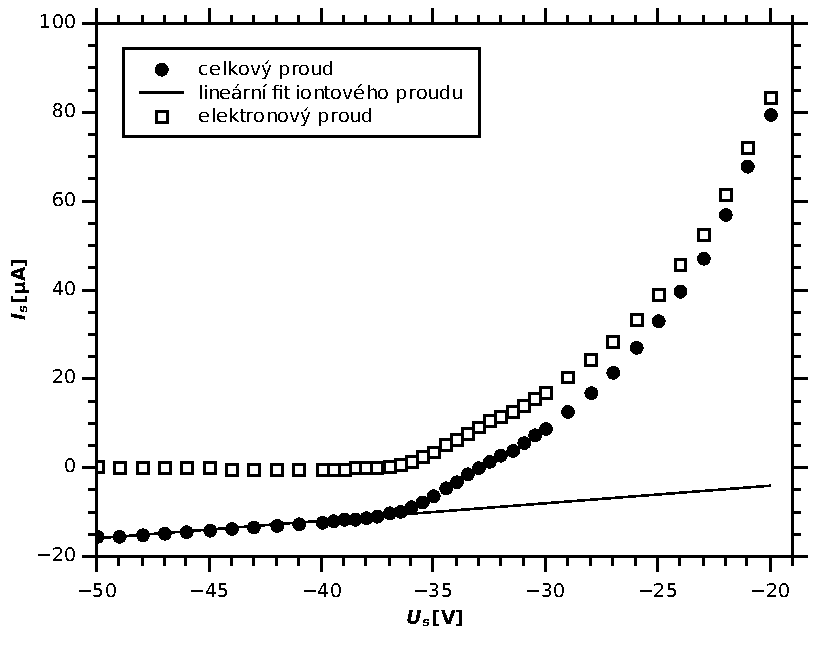
\includegraphics[width=11cm]{proudiv45.pdf}
\caption{Proud sondou s nafitovaným iontovým proudem a po odečtení iontového proudu pro $I_\mathrm{v}$ = 45\,mA}
\label{iv45}
\end{center}
\end{figure}

\begin{figure}[htbp]
\begin{center}
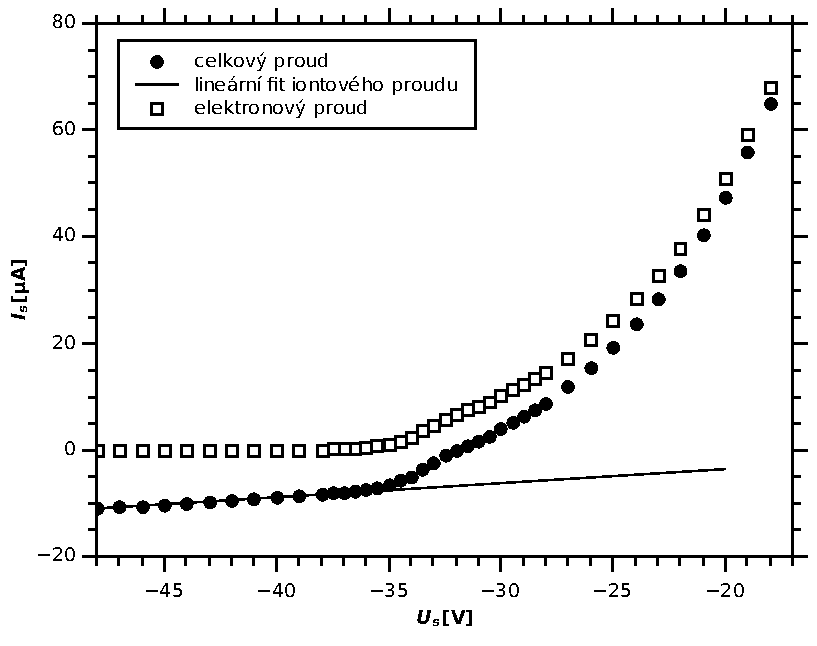
\includegraphics[width=11cm]{proudiv31.pdf}
\caption{Proud sondou s nafitovaným iontovým proudem a po odečtení iontového proudu pro $I_\mathrm{v}$ = 31\,mA}
\label{iv31}
\end{center}
\end{figure}

\begin{figure}[htbp]
\begin{center}
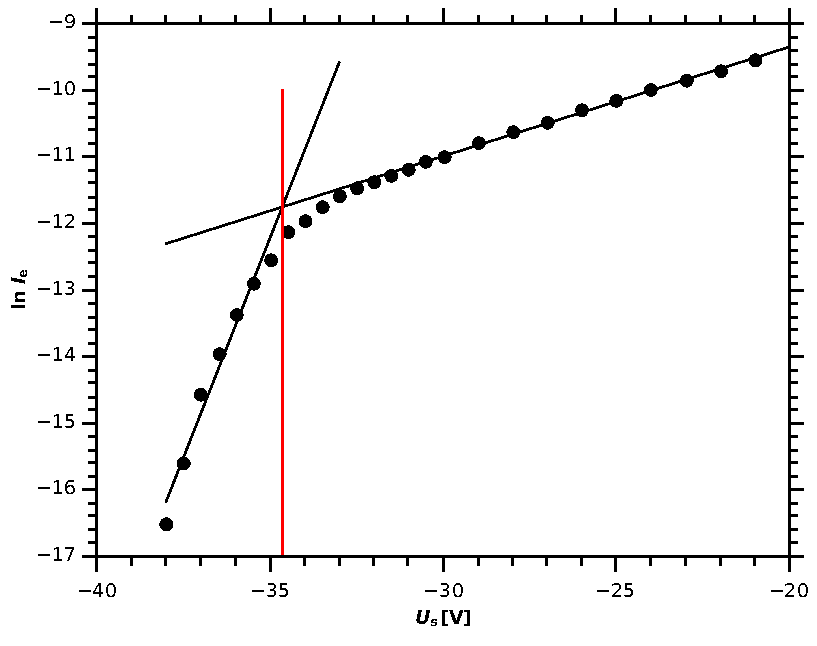
\includegraphics[width=11cm]{ln45.pdf}
\caption{Zlogaritmovaný elektronový proud s vyznačeným potenciálem plazmatu a asymptotami pro~$I_\mathrm{v}$ = 45\,mA}
\label{ln45}
\end{center}
\end{figure}

\begin{figure}[htbp]
\begin{center}
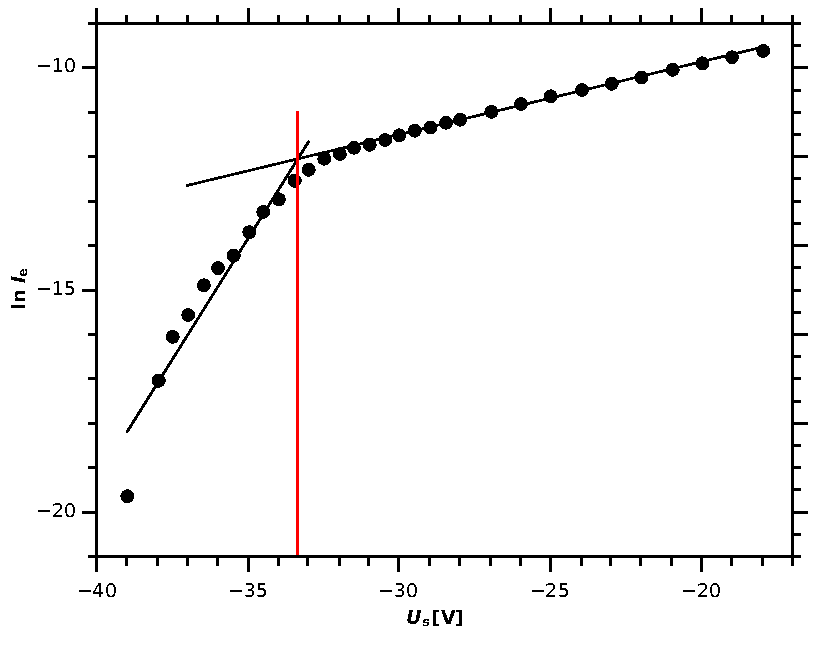
\includegraphics[width=11cm]{ln31.pdf}
\caption{Zlogaritmovaný elektronový proud s vyznačeným potenciálem plazmatu a asymptotami pro~$I_\mathrm{v}$ = 31\,mA}
\label{ln31}
\end{center}
\end{figure}

\begin{table}[htbp]
\begin{center}
\begin{tabular}{|c|c|c|c|c|c|}
\hline
$I_\mathrm{v}[\mathrm{mA}]$ & $U_\mathrm{fl}$[V] & $U_\mathrm{p}$[V] & $a$ & \boldmath$T_\mathrm{e} \mathrm{[K]}$ & $n_\mathrm{e}$[10${^{14}}$ m$^{-3}$] \\ \hline
45 & -33,1 & $-34,7\pm0,5$ & $1,32\pm0,12$ & \boldmath$8790\pm800$ & $1,69\pm1,79$ \\ \hline
31 & -32,0 & $-33,4\pm0,5$ & $1,08\pm0,10$ & \boldmath$10750\pm990$ & $1,27\pm1,34$ \\ \hline
\end{tabular}
\end{center}
\caption{Výsledky -- jednoduchá sonda}
\label{vysledkyjednoducha}
\end{table}

\subsection{Dvojná sonda}
Parametry sondového proudu byly určeny přímým odečtem z grafu získaného zapisovačem (v~pří\-lo\-ze). Na začátku bylo potřeba získat měřítko pro přepočet z centimetrů na ampéry a volty, to shrnuje obrázek \ref{prevod}. Měřítka jsou:
\begin{center}
x: $A_x = 1,004 \pm 0,005 \, \mathrm{V/cm}$\\
y: $A_y = 2,045 \pm 0,009 \, \mathrm{\mu A/cm}$
\end{center}

Následně byly určeny charakteristiky sondového proudu a z nich vypočítána teplota elektronů, to shrnuje tabulka \ref{vysledkydvojna}. Chyby přepočtu z centimetrů na ampéry a volty byly určeny z fitu, chyby při odečítání ze zakresleného grafu jsem dělal odhadem (většinou se jednalo řádově o 1--3\,mm). Ostatní chyby byly spočítány podle zákona šíření chyb.

\begin{table}[htbp]
\begin{center}
\begin{tabular}{|c|c|c|}
\hline
 & $I_\mathrm{v} = 45\,[\mathrm{mA}]$ & $I_\mathrm{v} = 31\,[\mathrm{mA}]$ \\ \hline
$I_\mathrm{p1}$ [cm] & $9,1 \pm	0,3$ & $7,1 \pm 0,3 $\\ \hline
$I_\mathrm{p1}$ [$\mu$A] &	$18,61 \pm	0,62$ & $ 14,52 \pm 0,61 $\\ \hline
$I_\mathrm{p2}$ [cm] & $9,4 \pm	0,3$ & $ 6,9 \pm 0,3 $ \\ \hline
$I_\mathrm{p2}$ [$\mu$A] & $19,22 \pm 0,63$ & $  14,11 \pm 0,62 $ \\ \hline
$I_\mathrm{e2}$ [cm] & $8,8 \pm 0,4$ & $ 6,4 \pm 0,4 $ \\ \hline
$I_\mathrm{e2}$ [$\mu$A] & $17,99 \pm 0,82$ & $ 13,09 \pm 0,81 $ \\ \hline
$\mathrm{d}I_\mathrm{d}$ [cm] & $7,6 \pm 0,2$ & $ 5,8 \pm 0,2 $ \\ \hline			
$\mathrm{d}I_\mathrm{d}$ [$\mu$A] & $15,54 \pm 0,41$ & $ 11,86 \pm 0,41 $ \\ \hline
$\mathrm{d}U_\mathrm{d}$ [cm] & $2,6 \pm 0,1$ & $ 2,6 \pm 0,1 $ \\ \hline
$\mathrm{d}U_\mathrm{d}$ [V] & $2,6 \pm 0,1$ & $ 2,6 \pm 0,1 $ \\ \hline
$\sum_{I_\mathrm{p}}$ [$\mu$A] & $37,83 \pm 0,87$ & $28,63 \pm 0,87$ \\ \hline
$R_0$ [10$^3$V/A] &	$167,9 \pm 7,9$ & $220,1 \pm 11,4$ \\ \hline
$G$ & $0,475 \pm 0,024$ & $0,457 \pm 0,031$ \\ \hline
\boldmath$T_\mathrm{e} [\mathrm{K}]$ & \boldmath$18380 \pm 970$ & \boldmath$18100 \pm 1100$ \\ \hline
\end{tabular}
\end{center}
\caption{Výsledky -- dvojná sonda}
\label{vysledkydvojna}
\end{table}


\begin{figure}[htbp]
\begin{center}
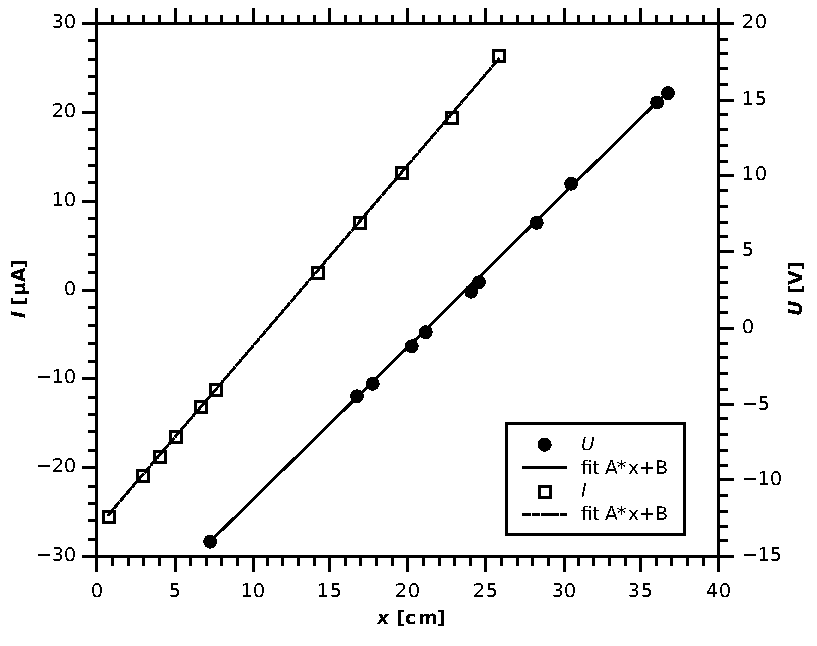
\includegraphics[width=11cm]{prevod.pdf}
\caption{Kalibrační křivky pro odečítání z grafu získaného zapisovačem}
\label{prevod}
\end{center}
\end{figure}

\section{Závěr}
Měření proběhlo úspěšně. Podařilo se určit elektronovou teplotu a koncentraci pro dva různé výbojové proudy. Elektonová teplota kolem 10000\,K naměřená jednoduchou sondou se mi zdá poněkud málo, ale alespoň řádově odpovídá očekáváním. Její chyba je asi 10\,\%, ale reálně mohla být ještě vyšší kvůli výše zmíněné nejednoznačnosti proložení asymptoty. Měření navíc muselo být zatíženo nějakou hrubou chybou, která způsobila, že plazmový potenciál vyšel pod plovoucím potenciálem, což je v přímém rozporu s teorií. Elektronová koncentrace je vyloženě orientační, protože závisí na ploše sondy, která byla určována odhadem, ale opět alespoň řádově souhlasí. U~dvojné sondy bylo měření mírně přesnější. Elektronová teplota kolem $18000\,\mathrm{K} \pm6\,\%$ se mi zdá mnohem reálnější. Nicméně výsledky se navzájem nevylučují protože byly měřeny v jiných oblastech výbojové trubice. 


\end{document}
